\documentclass[a4paper]{article}
\usepackage[margin=1in]{geometry}
\usepackage[fontset=founder]{ctex}
\usepackage{anyfontsize}
\usepackage{amsmath}
\usepackage{graphicx}

\graphicspath{{../figures/}}

\title{\textbf{常用电子仪器+RC电路频率特性}}
\author{姚苏航\qquad PB22061220 \\ 庞宇乐\qquad PB22061166 \\ 实验时间: 2023年11月1日\qquad 座位号: 05}
\date{}

\begin{document}

    \maketitle


    \section{实验目的}\label{sec:}

    \noindent {(1)在实验中学习、了解并熟练掌握常用电子仪器直流稳压电源、交流毫伏表、交流信号源、数字万用表以及示波器等常用电子仪器的使用, 为今后的实验打下基础。}

    \noindent {(2)测量CAL方波信号, 初步掌握示波器的使用方法。同时, CAL方波信号具有稳定的频率和幅值, 通过比对测量结果和标称值, 可以检验仪器的准确性和稳定性, 确保后续的测量实验结果的精度和可信性。}

    \noindent {(3)研究RC低通电路的相关性质, 通过测量不同频率下输入和输出信号的幅值和相位, 探究RC低通电路的频率响应特性, 确定RC电路的截止频率和衰减等。}


    \section{实验原理}\label{sec:2}
    \subsection{方波信号测量}
    {示波器是一种用途广泛的电子仪器, 它既能直接显示信号波形, 又能对电信号各种参数进行测量。利用该特性, 可以在AC档与DC档下测量示波器本身的校准信号(CAL)。}\label{subsec:}

    \subsection{一阶RC低通电路}\label{subsec:rc}

    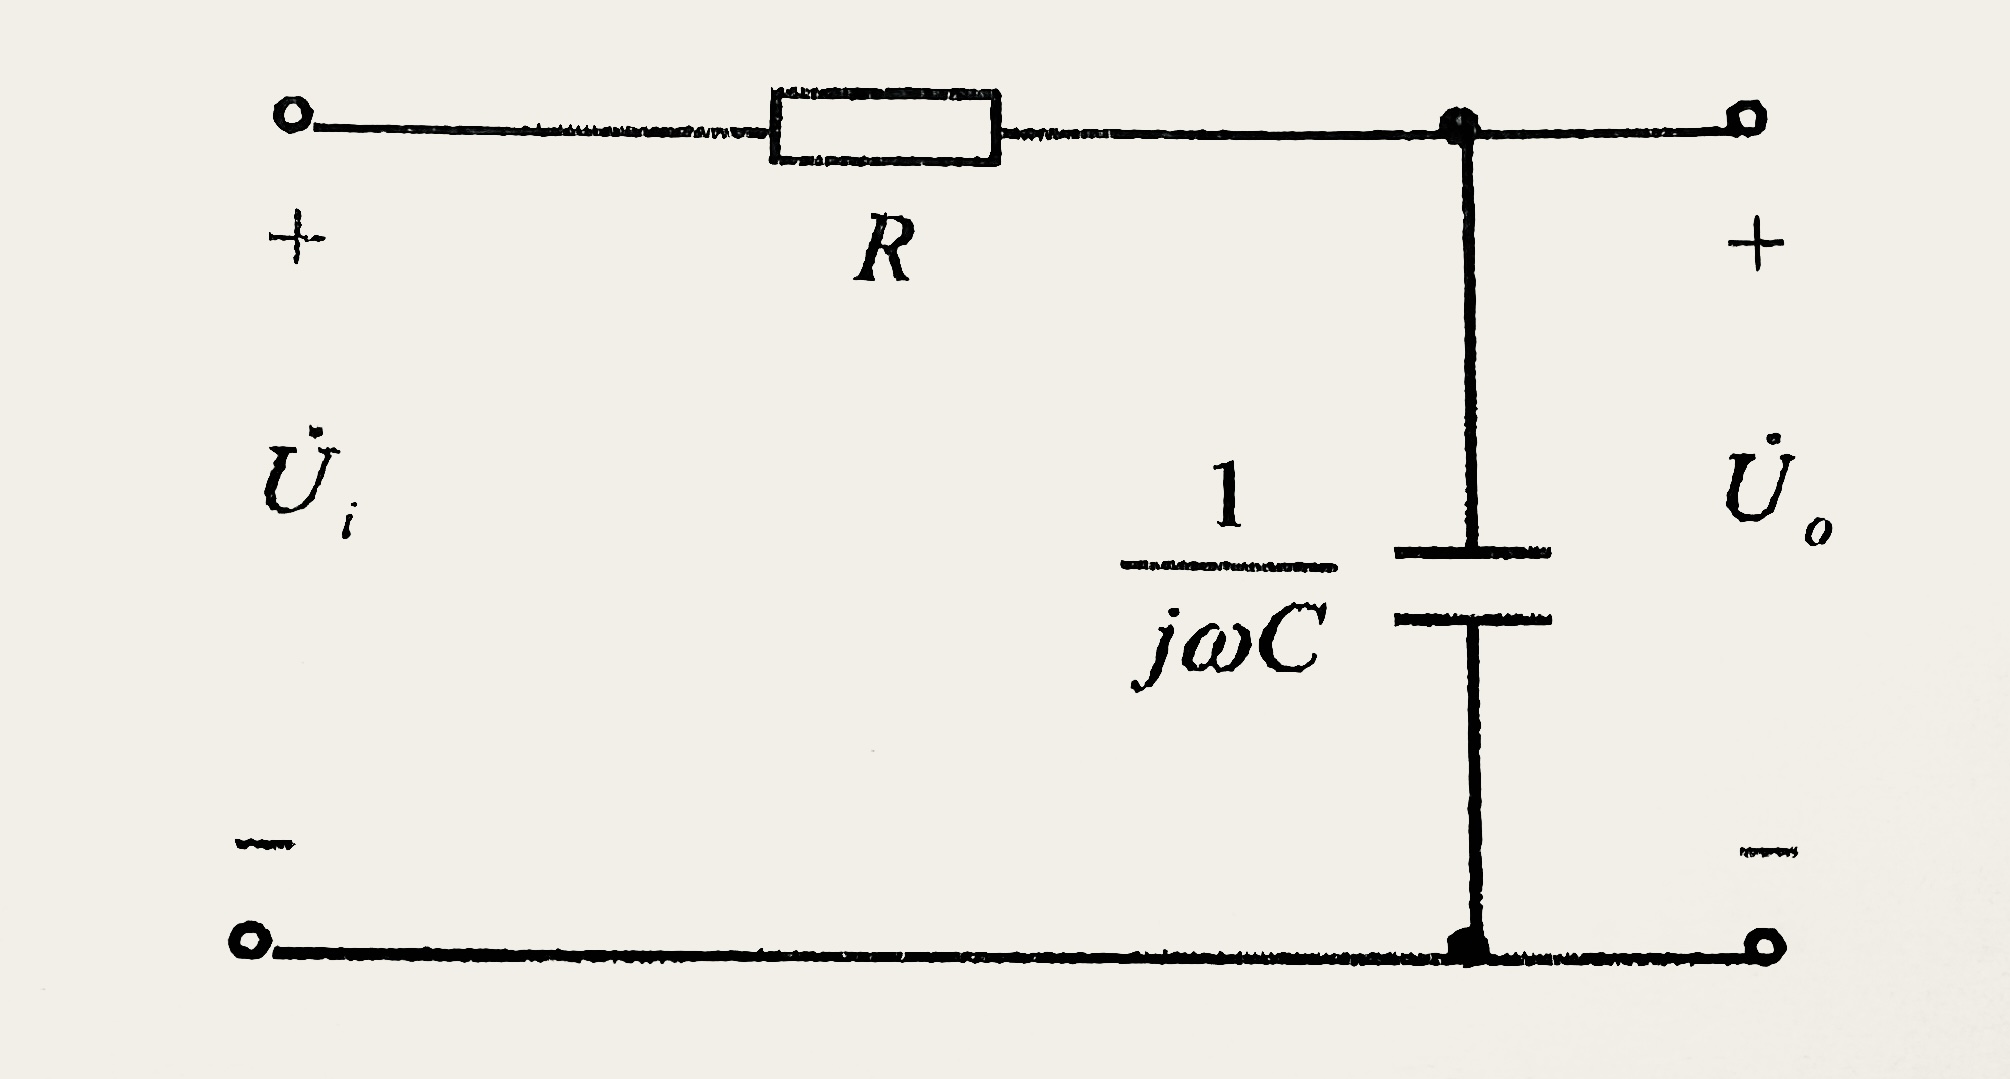
\includegraphics[height=0.2\textheight]{1}

    \hspace{3.5cm}{\small 图一}

    {如图为一阶RC低通电路。输出电压: $\stackrel{\cdot}{U_{o}}=\frac{\frac{1}{j \omega C}}{R+\frac{1}{j \omega C}}\stackrel{\cdot}{U_{i}}=\frac{\stackrel{\cdot}{U_{i}}}{j \omega R C+1}$}

    {其网络传递函数为: \[H(j \omega)=\frac{\stackrel{\cdot}{U_{o}}}{\stackrel{\cdot}{U_{i}}}=\frac{1}{j \omega R C+1}=\frac{1}{\sqrt{(\omega R C)^{2}+1}} \angle -tg^{-1}(\omega RC)=|H(j \omega)|\angle \phi(\omega)\]}

    {其中$|H(j \omega)|\stackrel{\Delta}{=}\frac{\stackrel{\cdot}{U_{o}}}{\stackrel{\cdot}{U_{i}}}=\frac{1}{\sqrt{(\omega R C)^{2}+1}}$, 表示输出与输入的幅值比, 称为幅值函数或增益函数, 幅值函数与频率的关系称为幅频特性, 显然是低通。$\angle \phi(\omega)=\angle -tg^{-1}(\omega RC)$。$\angle \phi(\omega)$表示输出与输入的相位差, 称为相位函数, 相位函数与频率的关系称为相频特性, 显然是输出滞后输入$\angle -tg^{-1}(\omega RC)$角度。}

    {当$\omega _{c}=\frac{1}{RC}$时, $|H(j \omega)|=\frac{1}{\sqrt{2}}$, $\phi (\omega)=-45^{\circ}$, 故$\omega _{c}(f_{c})$, 亦称为截止频率。对于低通电路, 频率0-$\omega _{c}(f_{c})$为通带, $\omega _{c}(f_{c})$-$\infty$为阻带。其频率特性如图2所示。}

    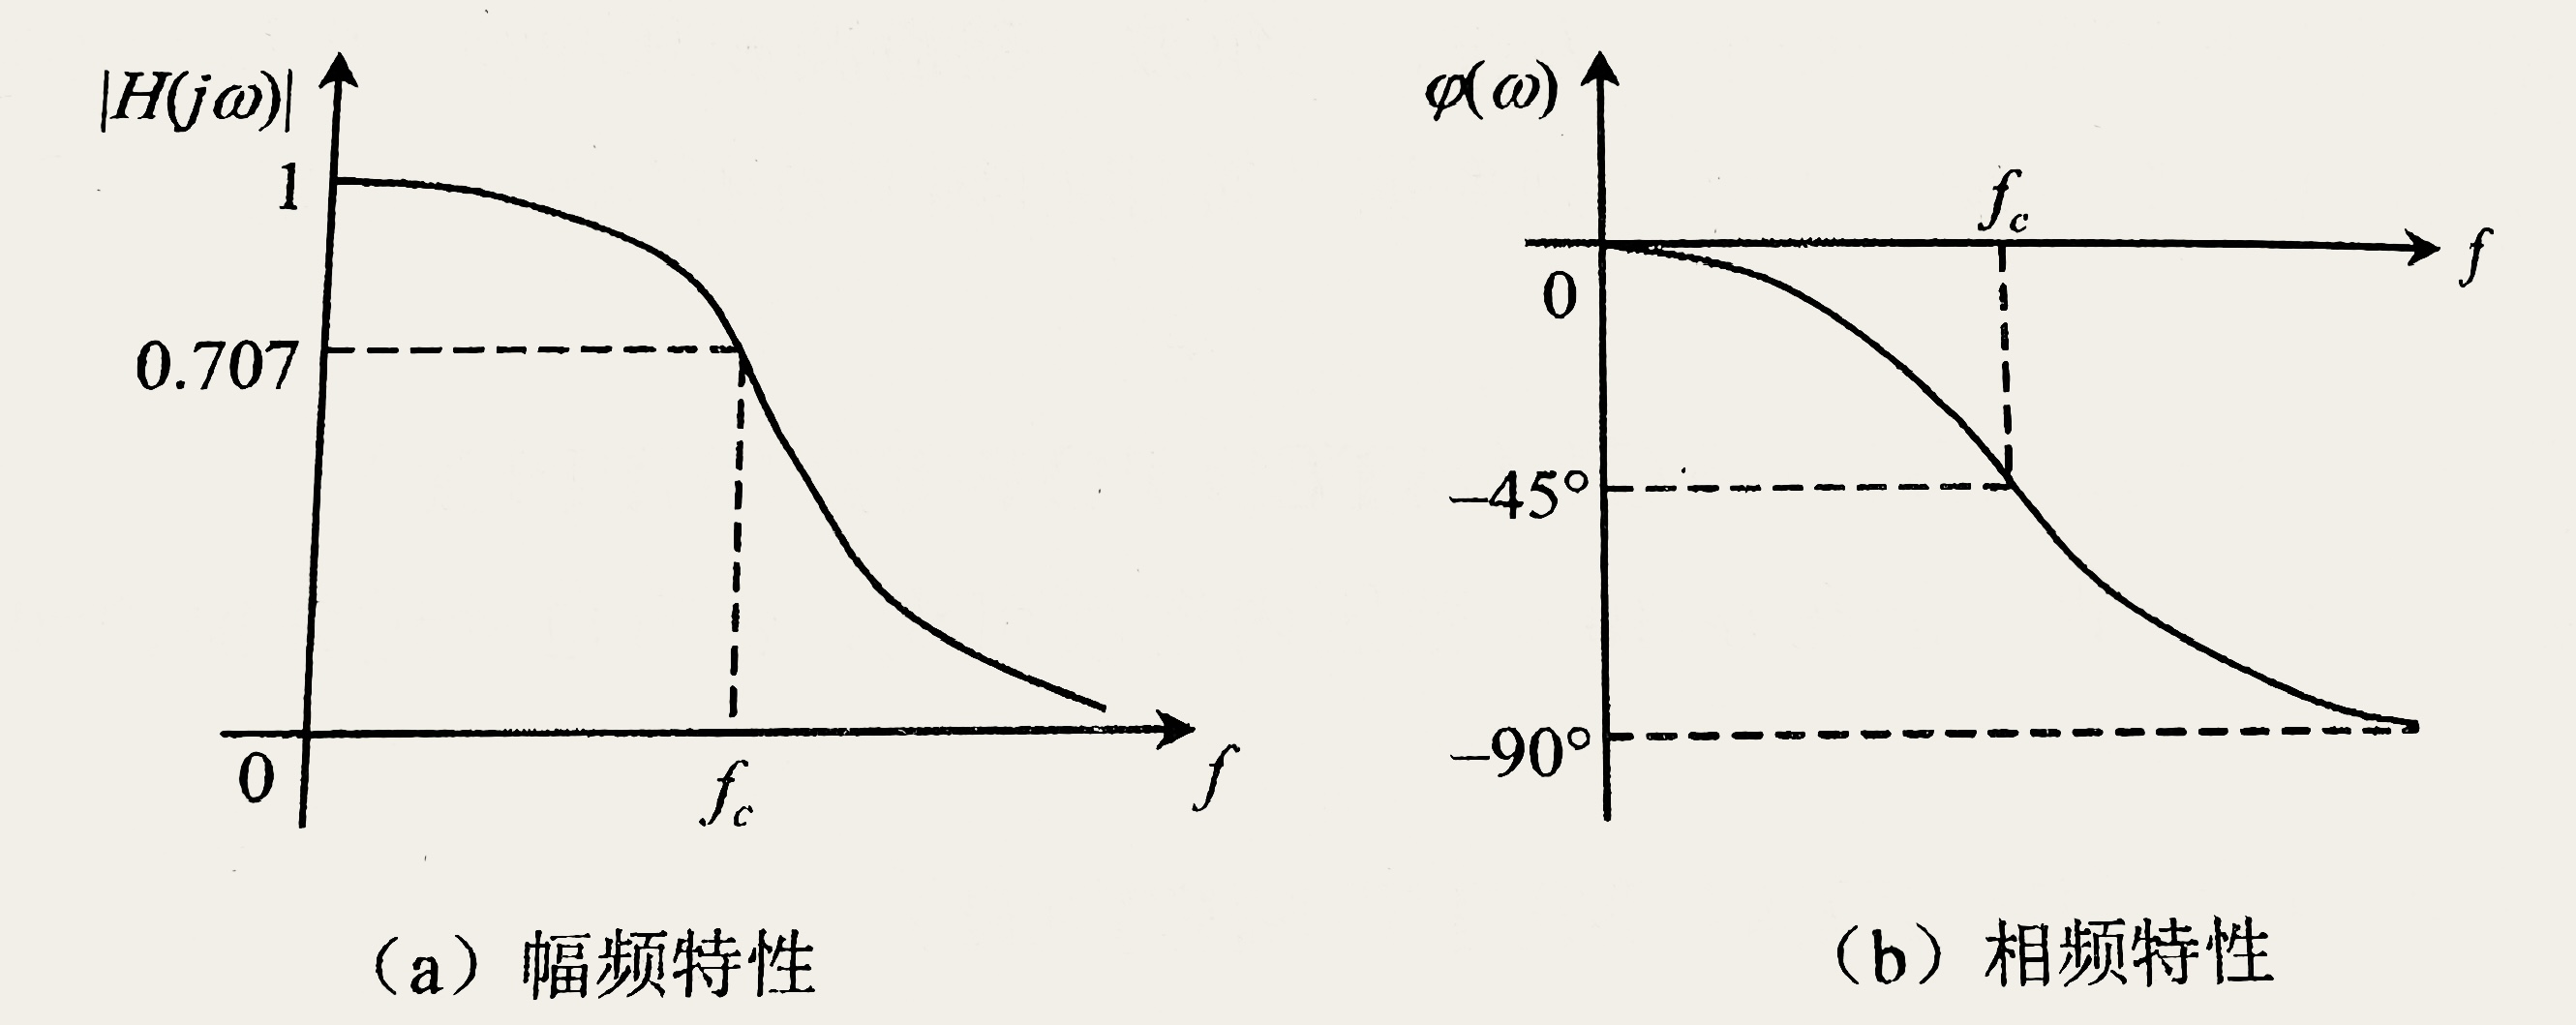
\includegraphics[height=0.22\textheight]{2}

    \hspace{5.3cm}{\small 图二}


    \section{实验内容与方法}\label{sec:3}
    \subsection{方波信号测量}

    {用$CH_{1}$(或$CH_{2}$)观测示波器本身的校准信号(CAL)用DC和AC档, 分别画出波形图, 在图上标出$U_{p}$, 和周期T。}\label{subsec:2}

    \subsection{一阶RC低通电路}

    {(1)按图1接线, 取$R=2.2k\Omega$,$C=0.1uF$,$U_{i}=1V$ (有效值)。测量输出电压, 并读取输出电压$U_{o}=0.707V$时的信号频率f, 用李沙育法测量相位差角。(接线之前, 先用万用表测量所用电阻和电容值, 理论计算时候代入万用表测量的, 不要代入标称值, 标称值误差太大) }

    {(2) 画出频率为工时的输入、输出电压波形图。并标明其超前、滞后的相位关系。}\label{subsec:rc2}

    \noindent{\textbf{相位差的测量方法: }}

    {图3 (a)为两信号李沙育图形, 它们之间相位差角$\phi =sin^{-1}\frac{B}{A}$, 式中A是李沙育图形在水平方向上的投影, B是李沙育图形在水平方向上两交点之间的距离。}

    {图3 (b)时域法根据两个同频率的正弦信号, 可以比较相位差。对于图中所示的两信号, 其之间的相位差角为$\phi=\frac{\Delta T}{T} \times 360^{\circ}$}

    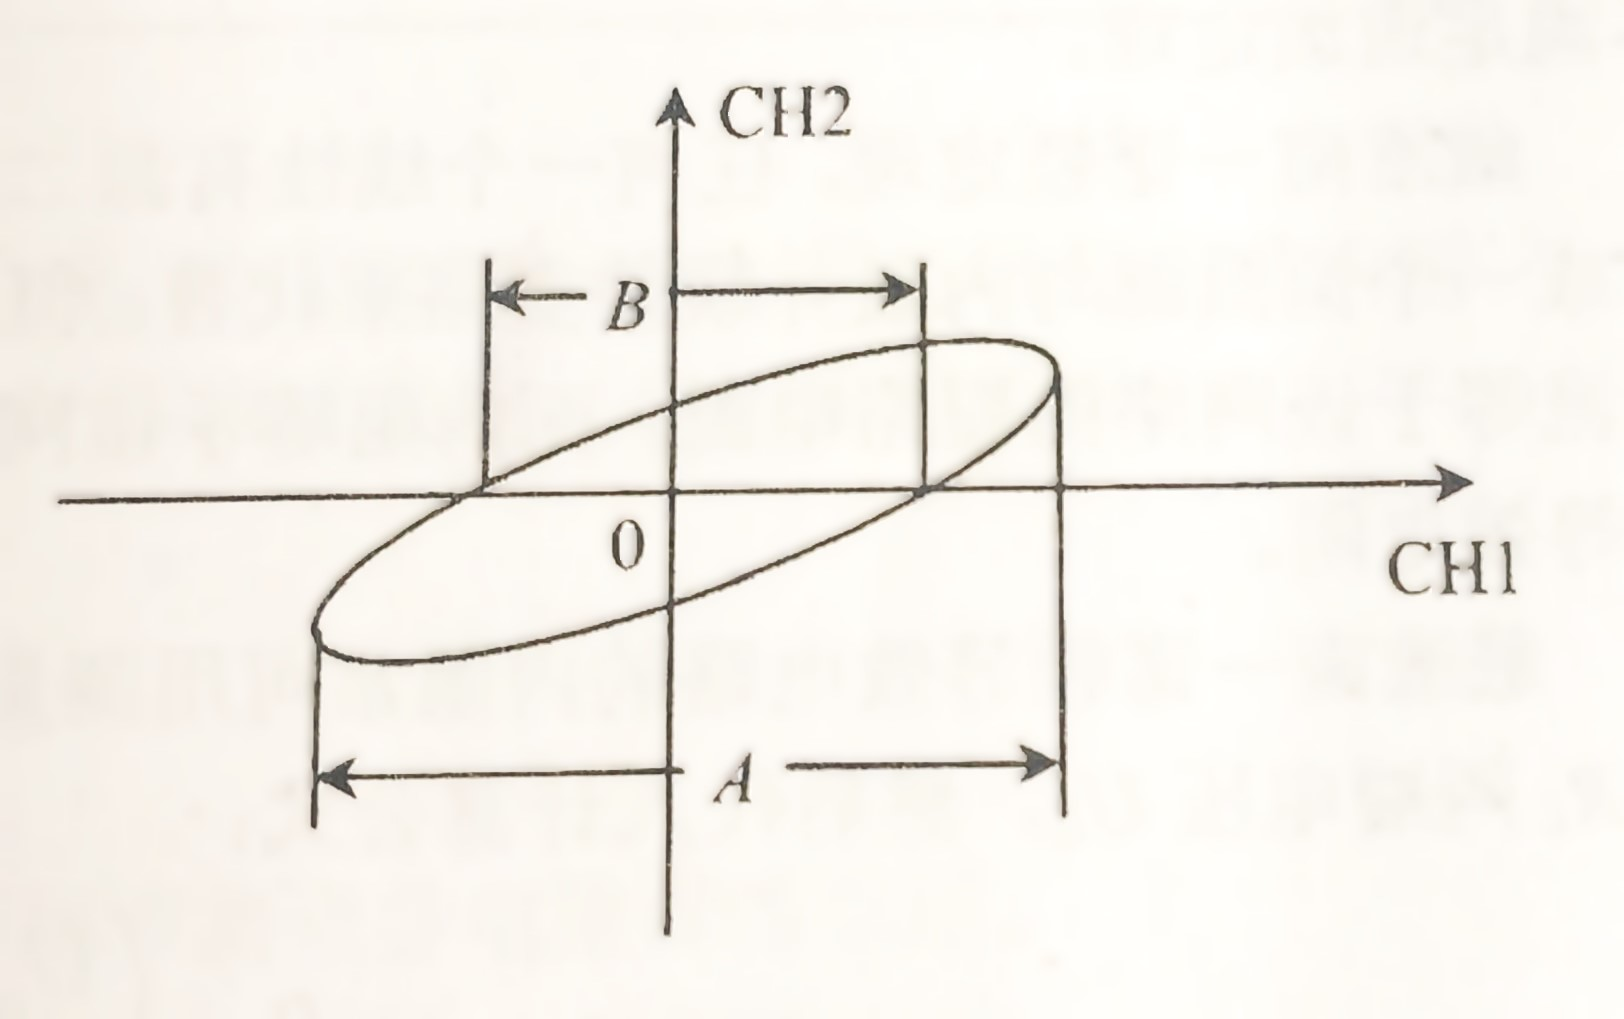
\includegraphics[height=0.20\textheight]{3}
    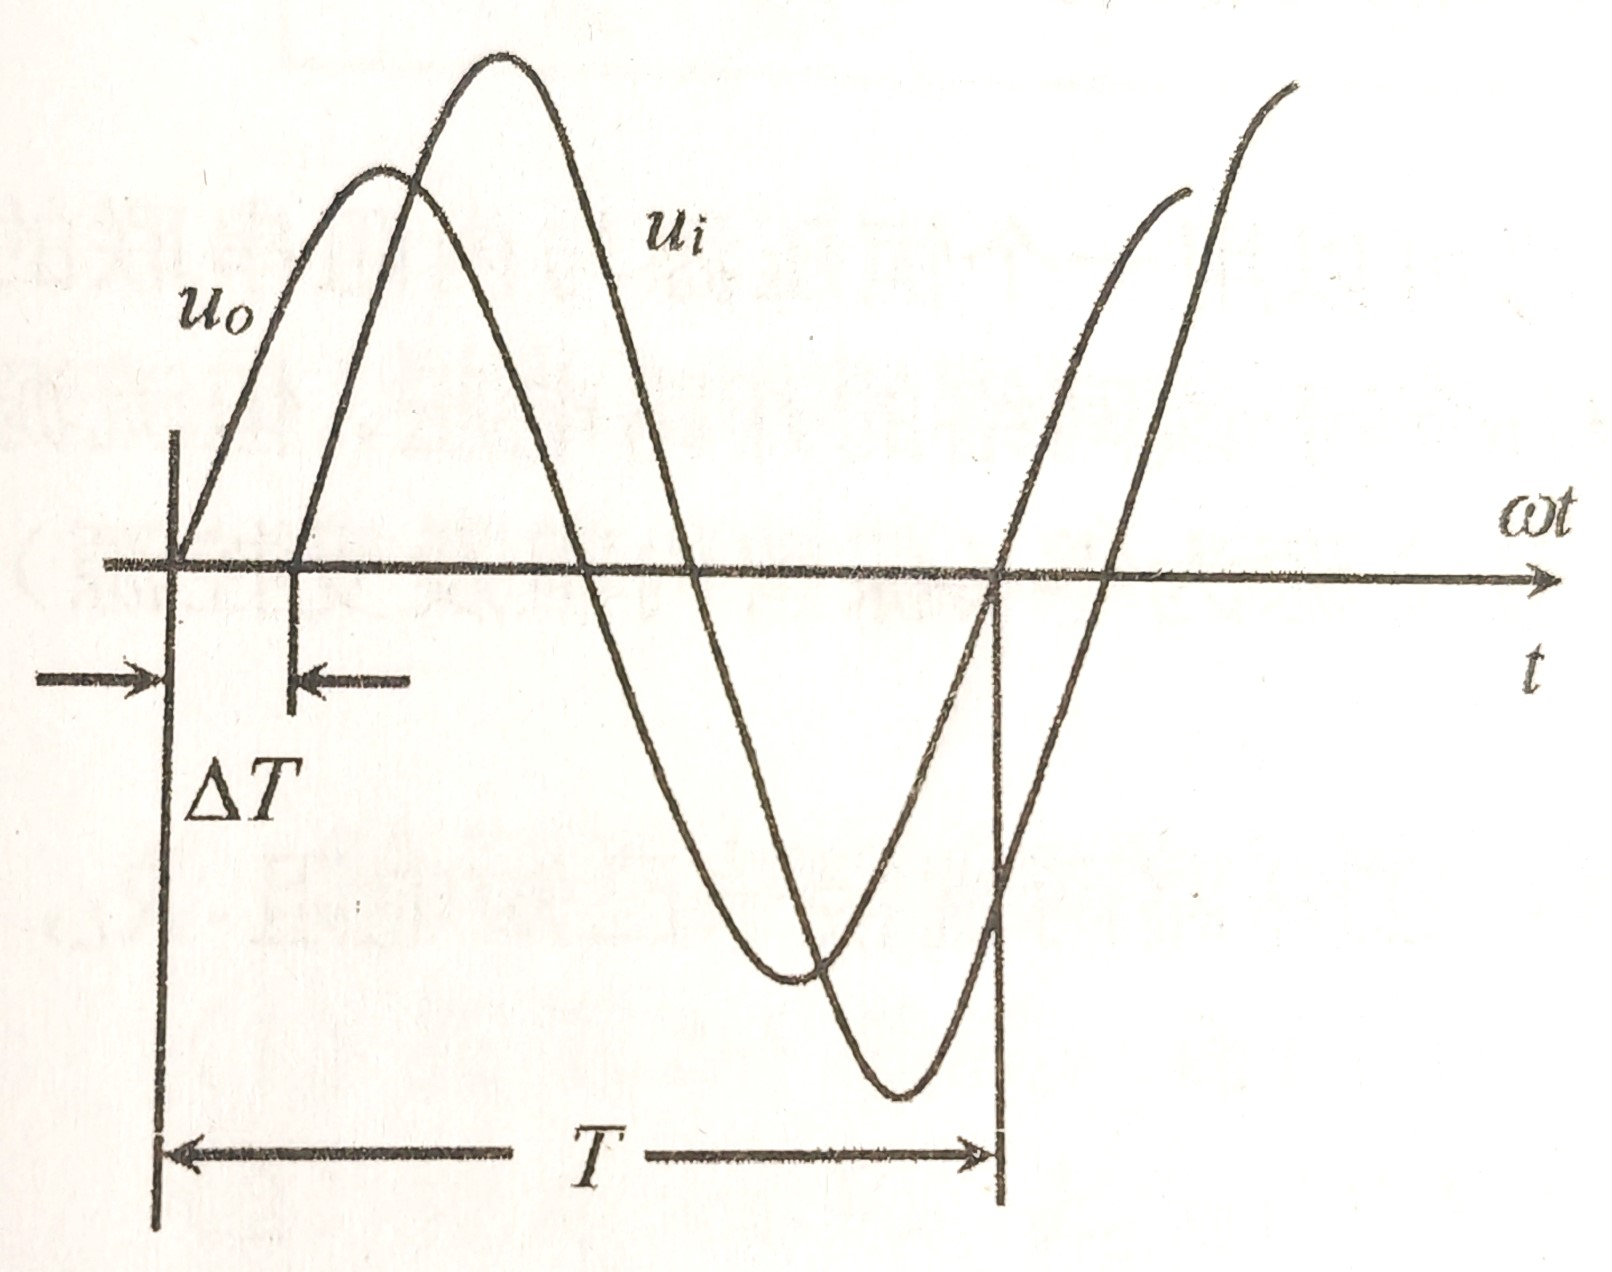
\includegraphics[height=0.21\textheight]{4}

    \hspace{2.8cm}{\small 图三 (a)}\hspace{4.8cm}{\small 图三 (b)}


    \section{实验数据与分析}\label{sec:4}

    \subsection{方波信号测量}\label{subsec:3}
    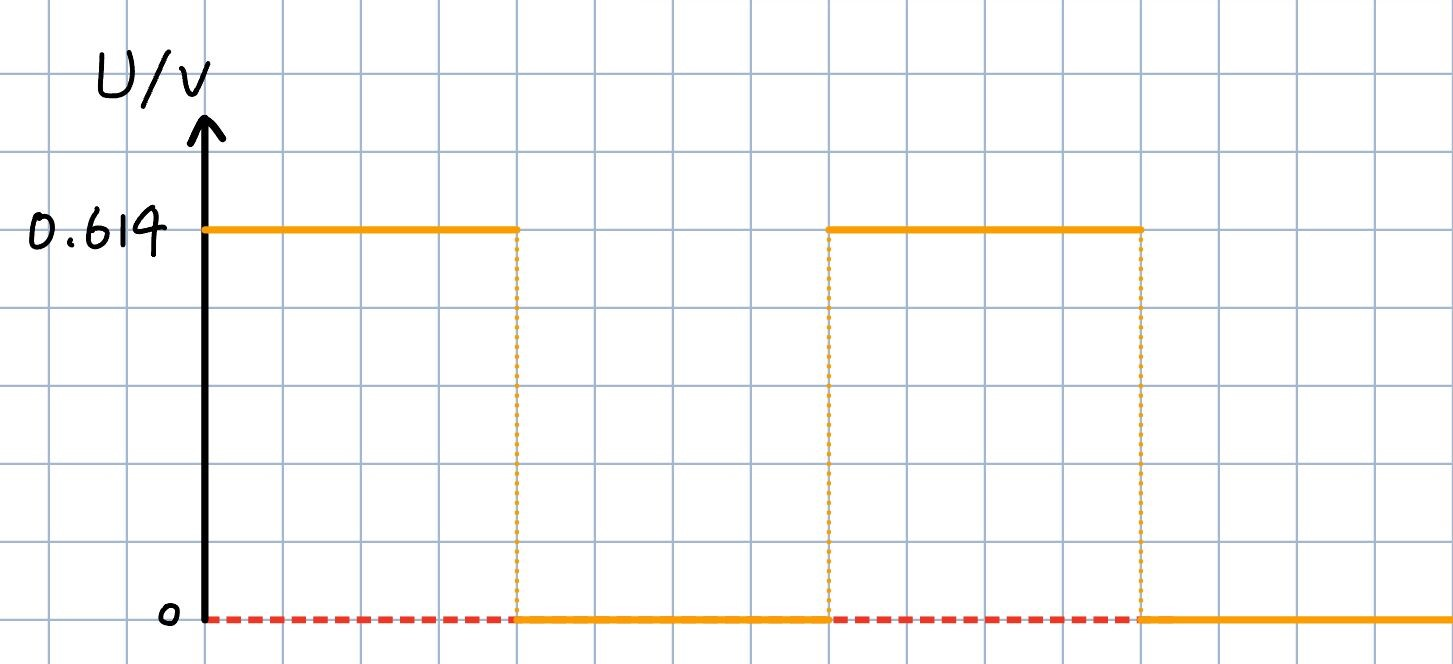
\includegraphics[height=0.13\textheight]{5}
    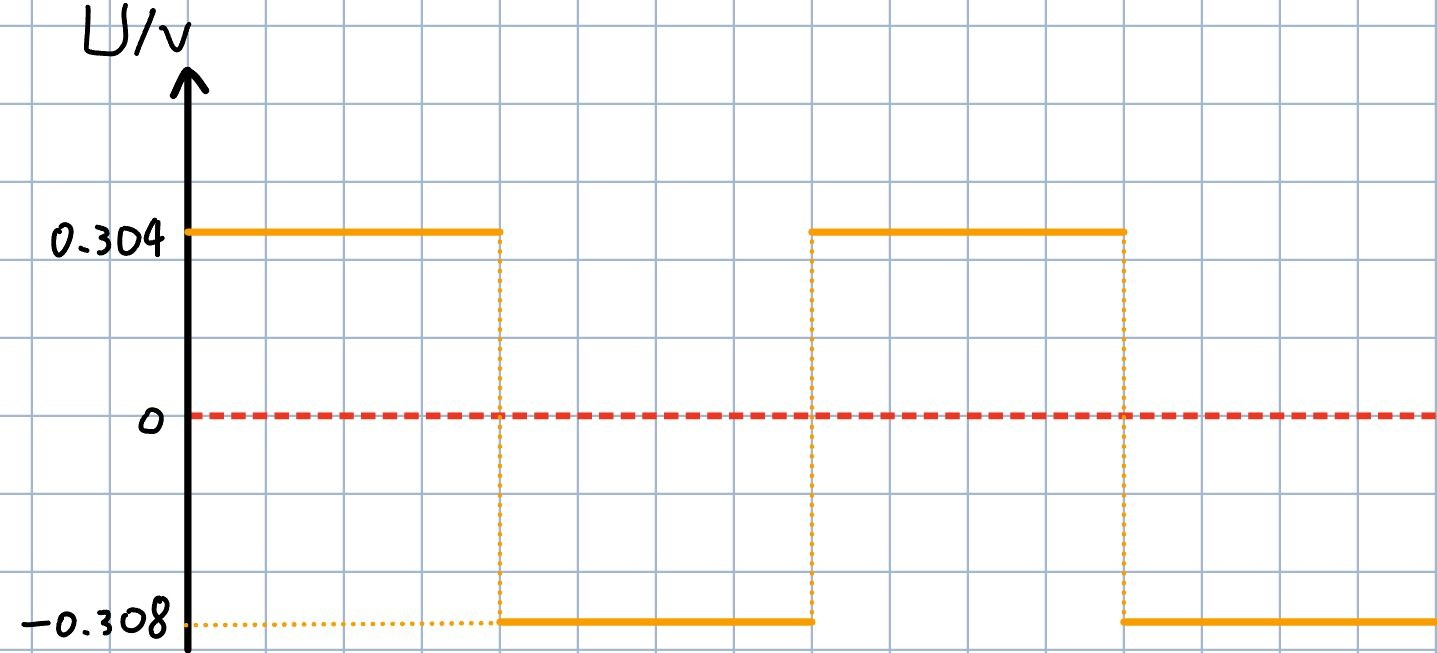
\includegraphics[height=0.13\textheight]{6}

    \hspace{2.7cm}{\small 图4}\hspace{4.9cm}{\small 图5}

    {图4为CAL方波DC档测量信号, 图5为CAL方波AC档测量信号。具体数据如下: }

    \begin{table}[htbp]
        \centering
        \caption{图4 数据}
        \begin{tabular}{|c|c|p{5cm}|}
            \hline
            CAL校准信号  & 标称值  & 测量值                         \\
            \hline
            幅度$U_{P-P}$ & 0.6V & $U_{P+}=0.614V$,$U_{P-}=0V$ \\
            \hline
            频率f         & 1kHz & $T=1.014ms$, $f=0.986kHz$   \\
            \hline
        \end{tabular}\label{tab:table}
    \end{table}

    \vspace{1cm}

    \begin{table}[htbp]
        \centering
        \caption{图5 数据}
        \begin{tabular}{|c|c|p{6cm}|}
            \hline
            CAL校准信号  & 标称值  & 测量值                              \\
            \hline
            幅度$U_{P-P}$ & 0.6V & $U_{P+}=0.304V$,$U_{P-}=-0.308V$ \\
            \hline
            频率f         & 1kHz & $T=1.014ms$, $f=0.986kHz$        \\
            \hline
        \end{tabular}\label{tab:table2}
    \end{table}

    \noindent{\textbf{数据(误差)分析: }}

    {在AC档下, 仪器采用交流耦合方式, 通过电容来消除直流分量, 只保留信号的交流成分。对于CAL方波信号的AC档测量, 仪器会忽略方波信号的直流分量, 当方波频率较低时, 方波信号会出现严重的失真。}

    {在DC档下, 仪器采用直流耦合方式, 相当于直接耦合, 对直流和交流成分均不加阻拦。对于CAL方波信号的DC档测量, 方波信号直接显示在示波器上, 失真较小。}

    {查阅资料可知, 根据奈奎斯特采样原理, 由于采样频率较低, 导致无法测量高频的电压信号, 在示波器上则显示为宽度较粗的方波信号, 也可能导致$U_{P+}$与$U_{P-}$失真。}

    \subsection{一阶RC低通电路}\label{subsec:rc3}

    \noindent{($R$应取$2.2K\Omega$, $C$应取$0.1mF$;由于仪器误差的存在, 最后实际数值为$R=2198.6\Omega,C=0.0998\mu F$; 上表中$\phi=sin^{-1}\frac{B}{A}$)}

    \begin{tabular}{|c|c|c|c|c|c|c|}
        \hline
        $f$($Hz$)        & 100      & 200    & 500    & 700    & 715    & 720    \\
        \hline
        $U_{i}$($V$)       & 0.993    & 0.986  & 0.983  & 0.972  & 0.976  & 0.969  \\
        \hline
        $U_{o}$($V$)       & 0.976    & 0.948  & 0.799  & 0.700  & 0.693  & 0.682  \\
        \hline
        $B$($V$)           & 0.375    & 0.700  & 1.520  & 1.845  & 1.86   & 1.895  \\
        \hline
        $A$($V$)           & 2.715    & 2.705  & 2.685  & 2.670  & 2.685  & 2.680  \\
        \hline
        $\phi$($^{\circ}$) & \, 7.939 & 14.998 & 34.479 & 43.710 & 44.367 & 44.999 \\
        \hline
    \end{tabular}

    \begin{tabular}{|c|c|c|c|c|c|c|}
        \hline
        $f$($Hz$)        & 725    & 740    & 800    & 1K     & 2K     & 5k     \\
        \hline
        $U_{i}$($V$)       & 0.976  & 0.972  & 0.976  & 0.979  & 0.965  & 0.962  \\
        \hline
        $U_{o}$($V$)       & 0.693  & 0.682  & 0.658  & 0.569  & 0.339  & 0.146  \\
        \hline
        $B$($V$)           & 1.87   & 1.915  & 1.96   & 2.145  & 2.45   & 2.59   \\
        \hline
        $A$($V$)           & 2.685  & 2.665  & 2.670  & 2.665  & 2.675  & 2.69   \\
        \hline
        $\phi$($^{\circ}$) & 44.140 & 45.937 & 47.230 & 53.598 & 66.332 & 74.238 \\
        \hline
    \end{tabular}

    \vspace{0.3cm}

    \noindent{由上表易知$f_{c}=720Hz, \phi=44.999^{\circ}$, 此时输入输出电压波形图如下所示。}

    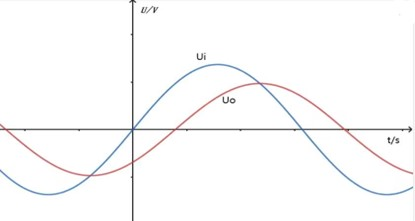
\includegraphics[height=0.18\textheight]{7}

    \hspace{2.5cm}{\small 图6}

    {根据测量数据绘制幅频(a)、相频特性(b)曲线如下图所示。}

    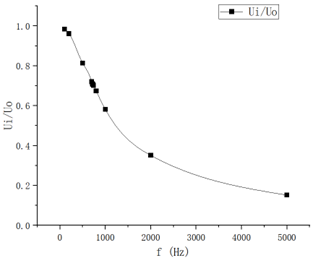
\includegraphics[height=0.20\textheight]{12}
    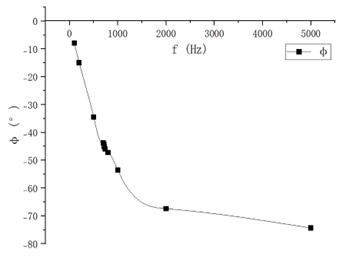
\includegraphics[height=0.20\textheight]{13}

    \hspace{1.5cm}{\small 图a 幅频特性图}\hspace{2.8cm}{\small 图b 相频特性图}

    \noindent{\textbf{理论计算: }}

    {理论上$\omega C=\frac{1}{R}$时, $f_{ideal}=\frac{1}{2\pi RC}=725.34Hz$, $U_{o}=\frac{U_{i}}{\sqrt{2}}$, 易知$U_{o}=0.685V$, $\phi=45^{\circ}$}

    {在实验过程中, $U_{i}$的值随着频率变化存在衰减, 因此频率$f_c$在$U_{o}=\frac{U_{i}}{\sqrt{2}}=0.685$时取到,而非在0.707V的理想值取得。}

    \vspace{0.5cm}

    \noindent{\textbf{数据(误差)分析: }}

    {(1) 当$U_{i}=0.969V$且, $f=720Hz$时, $U_{o}=0.682V$, $U_{o}$相对误差为\[\frac{U_{o}^{real}-U_{o}^{ideal}}{U_{o}^{ideal}}=0.348\%\]}

    {引起的可能原因是信号发生器存在内阻或电容、电阻值不精确。}

    {(2) 理论的$f_c=725.34Hz$, 实验中实际测得的$f_c=720Hz$, 相对误差为\[\delta=\frac{f^{real}-f^{ideal}}{f^{ideal}}=0.0074\%\]}

    {因此本次实验测量得到的截止频率相对误差较小, 较为准确。}

    {在实际电路中, 导线存在电阻, 因此实际测量得到的截止频率会小于理论计算出的截止频率, 这与本次实验的测量结果相符合。}

    {(3) $\phi$(李沙育图形法)相对误差为\[\frac{\phi^{real}-\phi^{ideal}}{\phi^{ideal}}=-0.002\%\]}

    {引起的可能原因是输入信号和输出信号之间的相位差随频率变化而变化, 而这种变化可能难以准确地反映在李萨如图形中(线条存在宽度导致测量不精确)。}

    {时域法和李萨如图形法测量截止频率下的相位差可能会有不同。因为它直接基于波形观察和时间差测量, 而李萨如图形法则受到输出信号幅值衰减的影响。故时域法更精确。}

    {上述误差均在误差允许范围内。}

    \vspace{1.7cm}


    \section{\textbf{思考题}}\label{sec:textbf}

    \noindent{\textbf{(1)两个不同频率的正弦信号能否测量其相位差, 为什么?}}

    {不能。若用时域法, 由于信号频率不同, 可能存在画面滚动等问题, 即在示波器屏幕上无法同时显示。并且信号频率不同导致时间差不断变化, 无法代入相应公式计算。}

    {而若采用李沙育图形法, 图像会呈现出复杂闭合曲线, 无法标定A与B, 亦无法计算。}

    {事实上, 不同频率的两个正弦量的相位差没有意义。对于两个不同频率的正弦波, 在不同时刻, 它们的相位差是不确定的, 即它们的相位差会随时间变化, 不具有稳定值。}

    \noindent{\textbf{(2)使用函数信号源时, 是接入电路调输入电压大小还是调好电压大小再接入电路?两者有何区别?}}

    {应先确定电压大小后接入电路, 再微调输入电压大小至预期值。}

    {先调节电压使接入电路的信号源输出的电压符合被测电路的输入要求, 避免因为过大的输出电压对电路或设备造成损害。}

    {但是, 由于信号源存在内阻以及电路本身分压等问题, 实际输出的电压与设定值会存在差距, 故电源电压无法代表路段电压$U_{i}$。接入电路后微调输入电压方可实现对$U_{i}$的精确控制。}

    \noindent{\textbf{(3)总结各种仪器的使用方法及注意事项。}}

    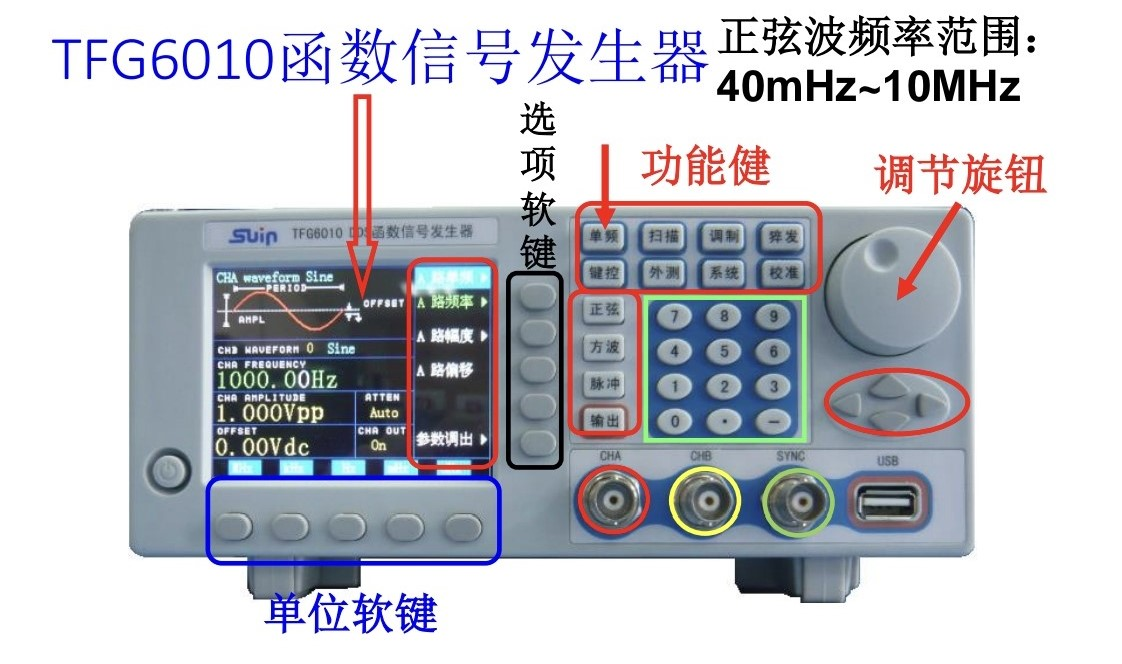
\includegraphics[height=0.18\textheight]{8}
    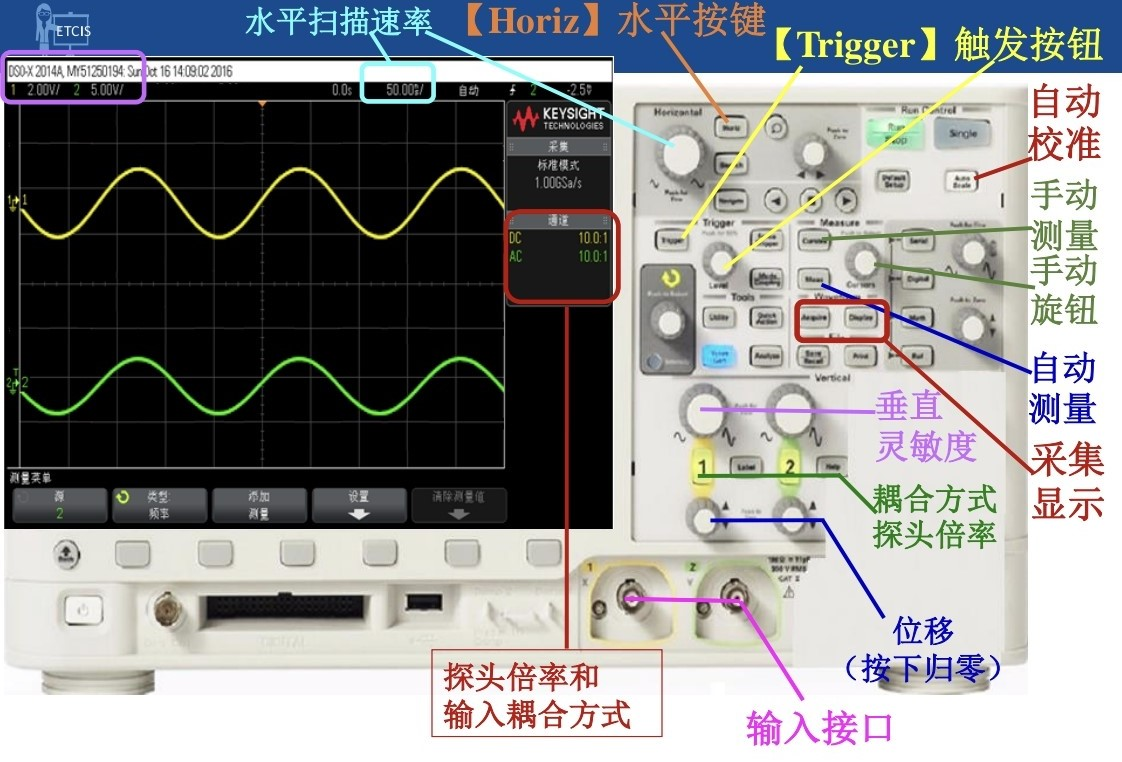
\includegraphics[height=0.18\textheight]{10}

    \hspace{2.5cm}{\small 图7}\hspace{4cm}{\small 图8}

    {图7为函数信号发生器, 能输出多种波形, 如正弦波、方波、三角波等。可为电路提供测试信号或作为标准源对一般信号进行校准比对。}

    \noindent{\textbf{使用方法: }}

    \noindent{(1)确保函数信号发生器的电源连接正确, 并进行良好的接地, 再将函数信号发生器的输出端与被测电路或设备的输入端连接;}

    \noindent{(2)根据实际需要, 选择函数信号发生器支持的信号类型, 如正弦波、方波、三角波、脉冲等;}

    \noindent{(3)根据实验要求, 设置所需的信号频率和幅值, 开启输出。}

    \noindent{\textbf{注意事项: }}

    \noindent{(1)输出线的两个夹子不能短路, 不能直接接到有较高直流电压的两点间;}

    \noindent{(2)与被测电路连接时, 红夹子接信号端, 黑夹子接地;}

    \noindent{(3)幅度读数不准确, 需要用相应的测量工具测量并记录;}

    \noindent{(4)屏幕上不直接显示B路波形, 由CHB WAVEFORM Sine显示;}

    \noindent{(5)注意信号源的输出功率限制, 避免过大的输出信号对电路或设备造成损坏.}

    \vspace{0.5cm}

    \noindent{图8为示波器, 可观察电信号时域波形与李沙育图形, 亦可测量电信号幅值。周期等参数。}

    \noindent{\textbf{使用方法: }}

    \noindent{(1)将示波器的探头正确地连接到被测电路或设备上, 并确保信号输入端和地端连接正确;}

    \noindent{(2)设置电信号, 接入合适测量通道;}

    \noindent{(3)按需设置水平轴与时间轴的尺度与偏移量。注意选择合适的时间刻度与电压刻度比例以获取更清晰的波形, 并通过调整水平位移和垂直位移, 以便得到合适的波形显示;}

    \noindent{(4)调节光标测量、实时测量、时基等模式, 获取所需图像。}

    \noindent{\textbf{注意事项: }}

    \noindent{(1)显示亮度应合适, 不应长时间显示固定亮点;}

    \noindent{(2)被测电压幅值(直流加交流的峰值)不应超过示波器的最大允许输入电压, 防止损坏仪器;}

    \noindent{(3)被测电压频率不应超过带宽值;}

    \noindent{(4)与被测电路连接时, 探针接信号端, 黑夹子接地;}

    \noindent{(5)读取波形参数时, 波形高度应超过屏幕高度的一半。}


    \vspace{1cm}


    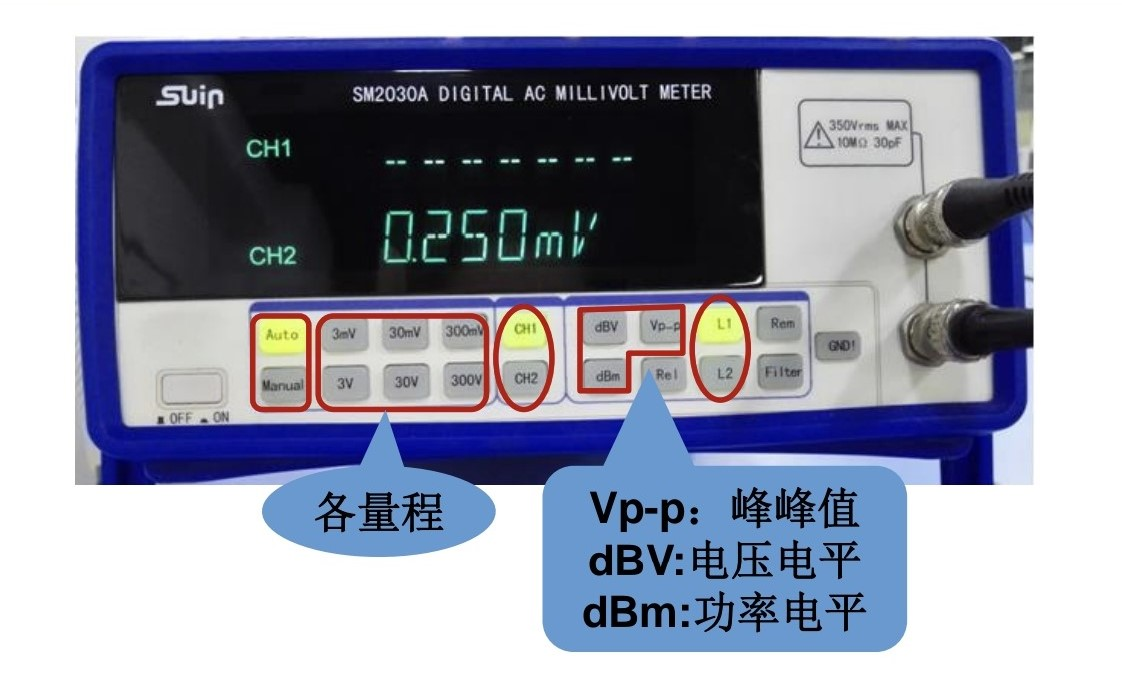
\includegraphics[height=0.17\textheight]{9}
    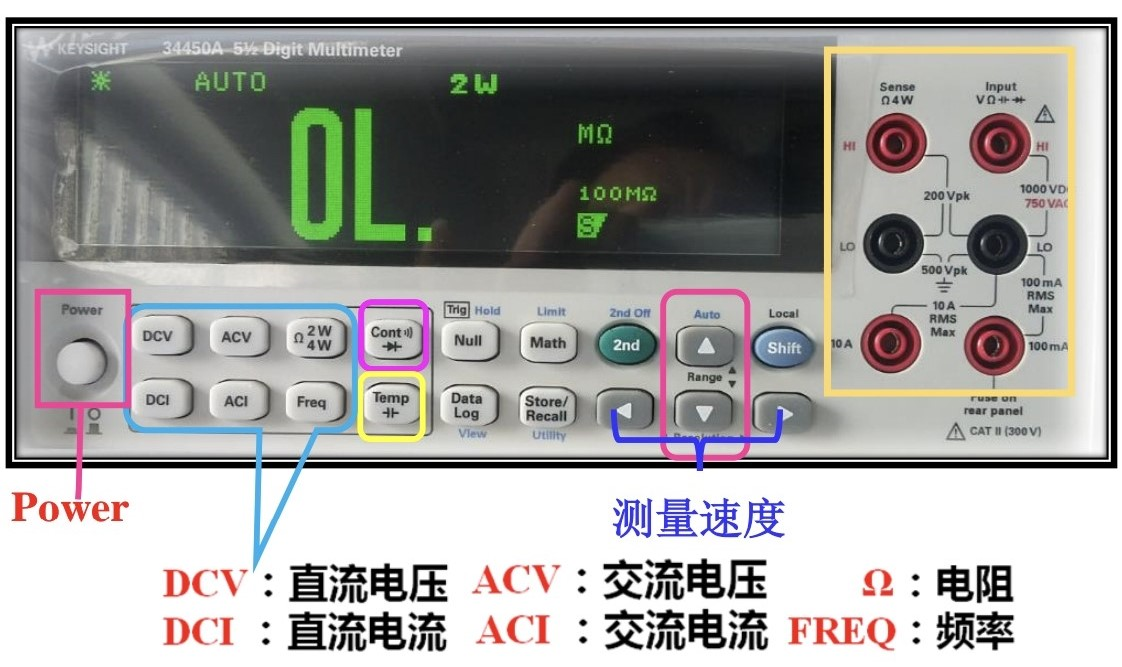
\includegraphics[height=0.165\textheight]{11}

    \hspace{2.5cm}{\small 图9}\hspace{4cm}{\small 图10}

    \noindent{图9为交流毫伏表, 可选择测量线路、测量对象与量程。}

    \noindent{\textbf{使用方法: }}

    \noindent{(1)在开始使用之前, 确保进行正确的校准;}

    \noindent{(2)根据待测电压的范围选择合适的量程档位。确保所选档位能够覆盖待测信号的幅值范围, 同时避免过量程而损坏仪器;}

    \noindent{(3)将交流毫伏表的输入端正确地连接到待测电路或电源的输出端;}

    \noindent{(4)打开交流毫伏表, 观察并记录所测量的交流电压值。}

    \noindent{\textbf{注意事项: }}

    \noindent{(1)应尽量选择小量程, 使实验测试数据更为精确;}

    \noindent{(2)了解交流毫伏表的内阻, 选择阻抗合适的测量对象;}

    \noindent{(3)在任何调整连接中, 确保电路处于安全状态。}

    \vspace{0.5cm}

    \noindent{图10为数字万用表, 可选择测量对象与量程。}

    \noindent{\textbf{使用方法: }}

    \noindent{(1)根据被测信号的预估数值, 选择合适的测量范围;}

    \noindent{(2)将测试引线分别连接到数字万用表上的相应插孔, 通常为红色正极和黑色负极;}

    \noindent{(3)测量相应对象。}

    \noindent{\textbf{注意事项: }}

    \noindent{(1)测量电阻时, 被测电阻不能带电;}

    \noindent{(2)测量电容时, 应先放电再测量;}

    \noindent{(3)被测电压值不应超过端口允许值, 交流电压频率不应超过带宽值;}

    \noindent{(4)测试前选择正确端口接入测试引线, 选择正确功能键、量程、分辨率/速度。}

    \noindent{(5)表笔接在"mA"与"A"时, 不能测量电压。}


    \section{实验总结}\label{sec:5}

    \noindent{(1)对本实验的示波器、稳压电源、函数信号发生器、毫伏表、万用表等仪器的使用方法有基本了解, 为今后的实验打下基础。}

    \noindent{(2)通过对CAL方波信号的测量, 我们得到了其频率、幅值等参数。实验结果显示, 测得的相关参数与标称值相符合, 说明仪器的测量精度和稳定性较好。因此, 我们成功地验证了仪器的准确性和稳定性, 确保示波器显示结果的精度和可信度处于允差范围内。}

    \noindent{(3)通过测量RC低通电路在不同频率下的输入和输出信号的幅值和相位差, 我们得到了RC低通电路的幅频响应特性与相频响应特性。实验结果表明, RC低通电路的输出信号随着频率的增加而逐渐衰减。此外, 通过电路的幅频特性, 我们可以确定RC低通电路的截止频率, 并验证了RC低通电路的滤波效果, 即可以有效滤除高频成分, 使得只有低频信号透过, 这与理论预期基本吻合。}

\end{document}